\documentclass{beamer}

\usepackage[utf8]{inputenc}
\usetheme{default}

\begin{document}

\begin{frame}
 Dataset:
 \begin{itemize}
  \item 5 patients weighted t1 and t2 for 176 slices
  \item Bicubic Downsampling 2x and 4x + gauss noise
  \item 2LR 128x128 and 4LR 64x64 
 \end{itemize}
 
Analysis:
 \begin{itemize}
  \item model edsr x2 128x128 $\rightarrow$ 256x256 RGB
  \item model wdsr x4  64x64  $\rightarrow$ 256x256 RGB 
  \item bicubic interpolation scale 2x and 4x
  \item rotation of 20 angles for super-resolution
  \item PSNR and SSIM score by channels 
  \item Evaluate SR and its limits
 \end{itemize}

\end{frame}

%\begin{frame}
  %\begin{figure}
  %\includegraphics[scale=0.25]{images/%ref_case01015_t1_2lr_100_000.png}
 %\end{figure}
%\end{frame}

%\begin{frame}
  %\includegraphics[scale=0.25]{images/%ref_case01015_t1_4lr_100_018.png}
%\end{frame}
  
\begin{frame}
\frametitle{EDSR results per slice}
  \begin{figure}
  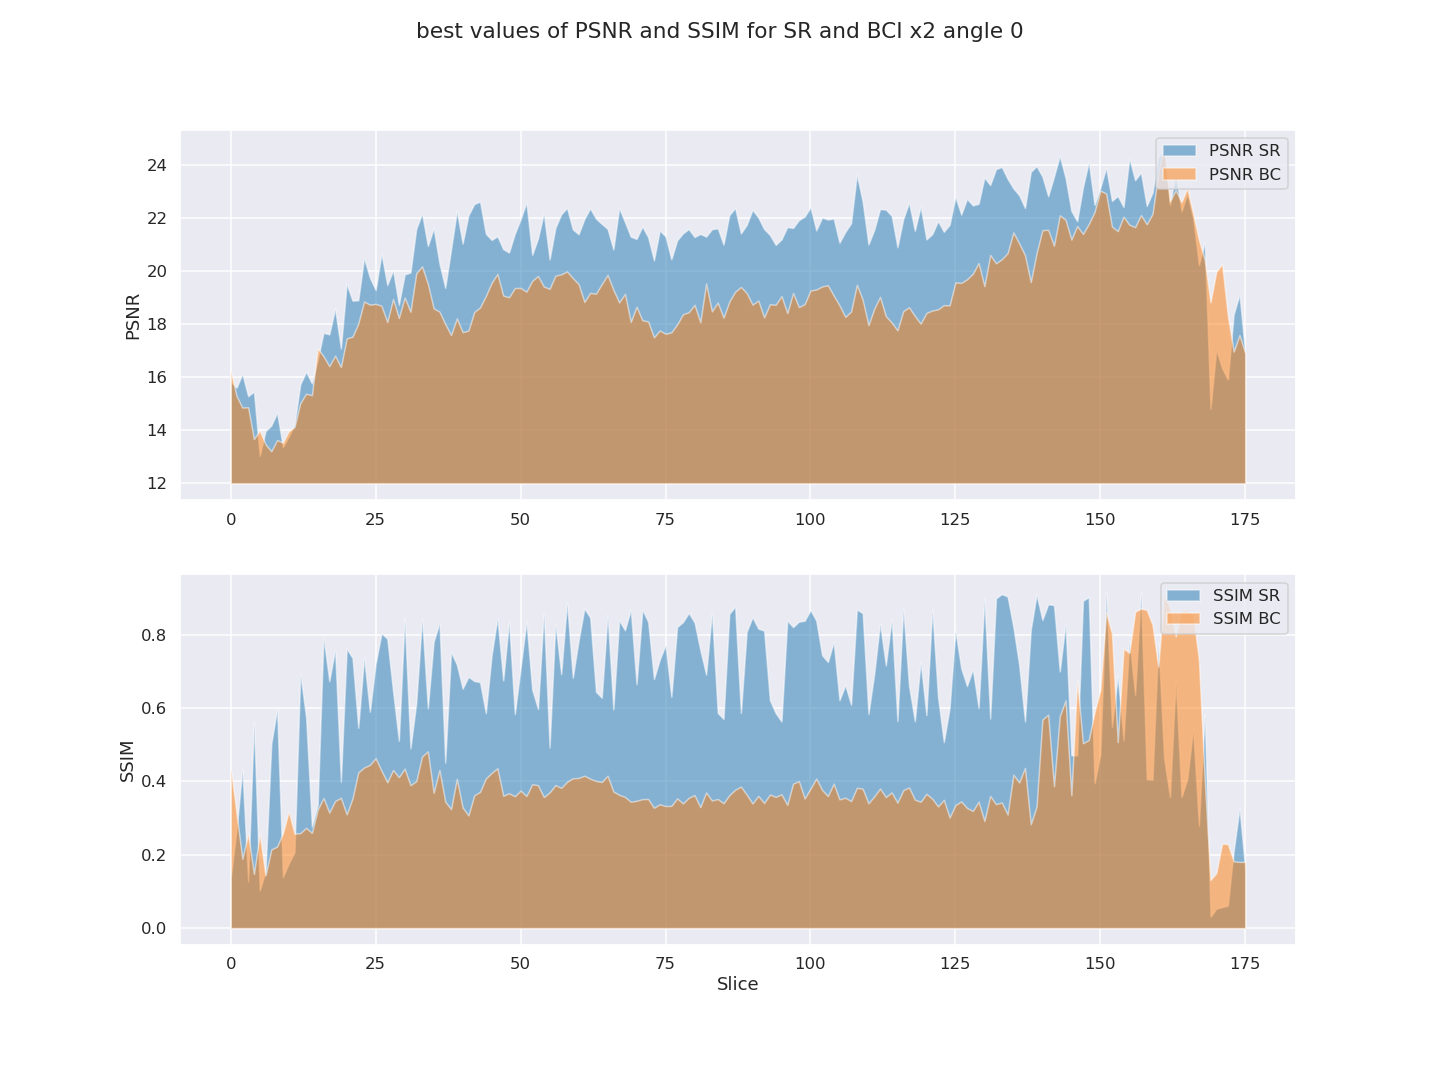
\includegraphics[scale=0.22]{images/PSNR-SSIM_sr-bc_x2_000.png}
 \end{figure}
\end{frame}

\begin{frame}
  \frametitle{Frames References: slice 25 and slice 153}
    \begin{figure}
  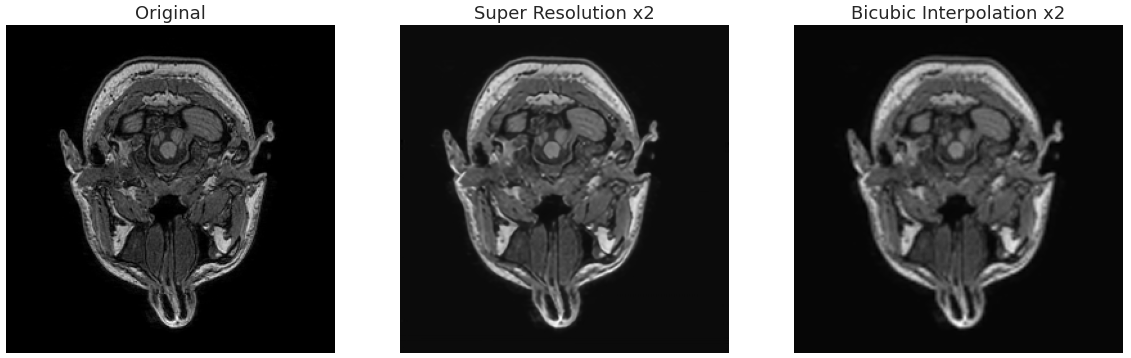
\includegraphics[scale=0.29]{images/ref_case01015_t1_2lr_025_000.png}
  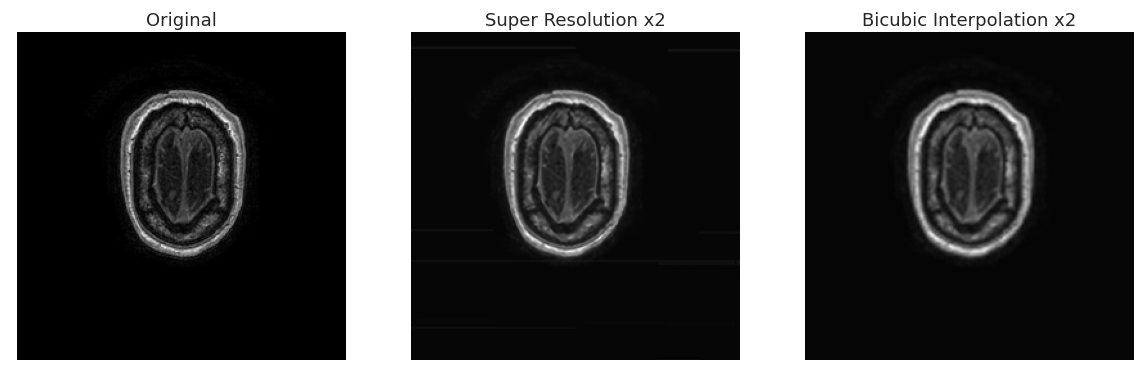
\includegraphics[scale=0.29]{images/ref_case01015_t1_2lr_153_000.png}
 \end{figure}
\end{frame}

\begin{frame}
 \frametitle{A central slice}
 \begin{figure}
  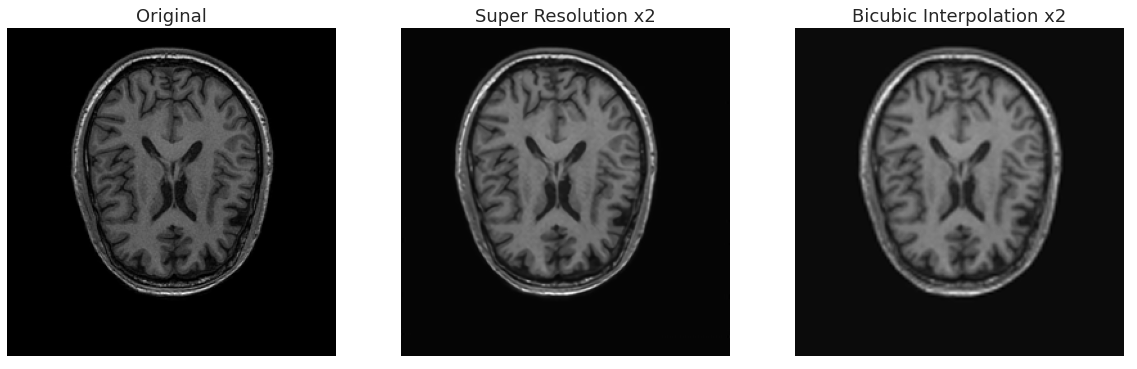
\includegraphics[scale=0.29]{images/ref_case01015_t1_2lr_100_000.png}
 \end{figure}
\end{frame}


\begin{frame}
\frametitle{WDSR results per slice  }
   \begin{figure}
  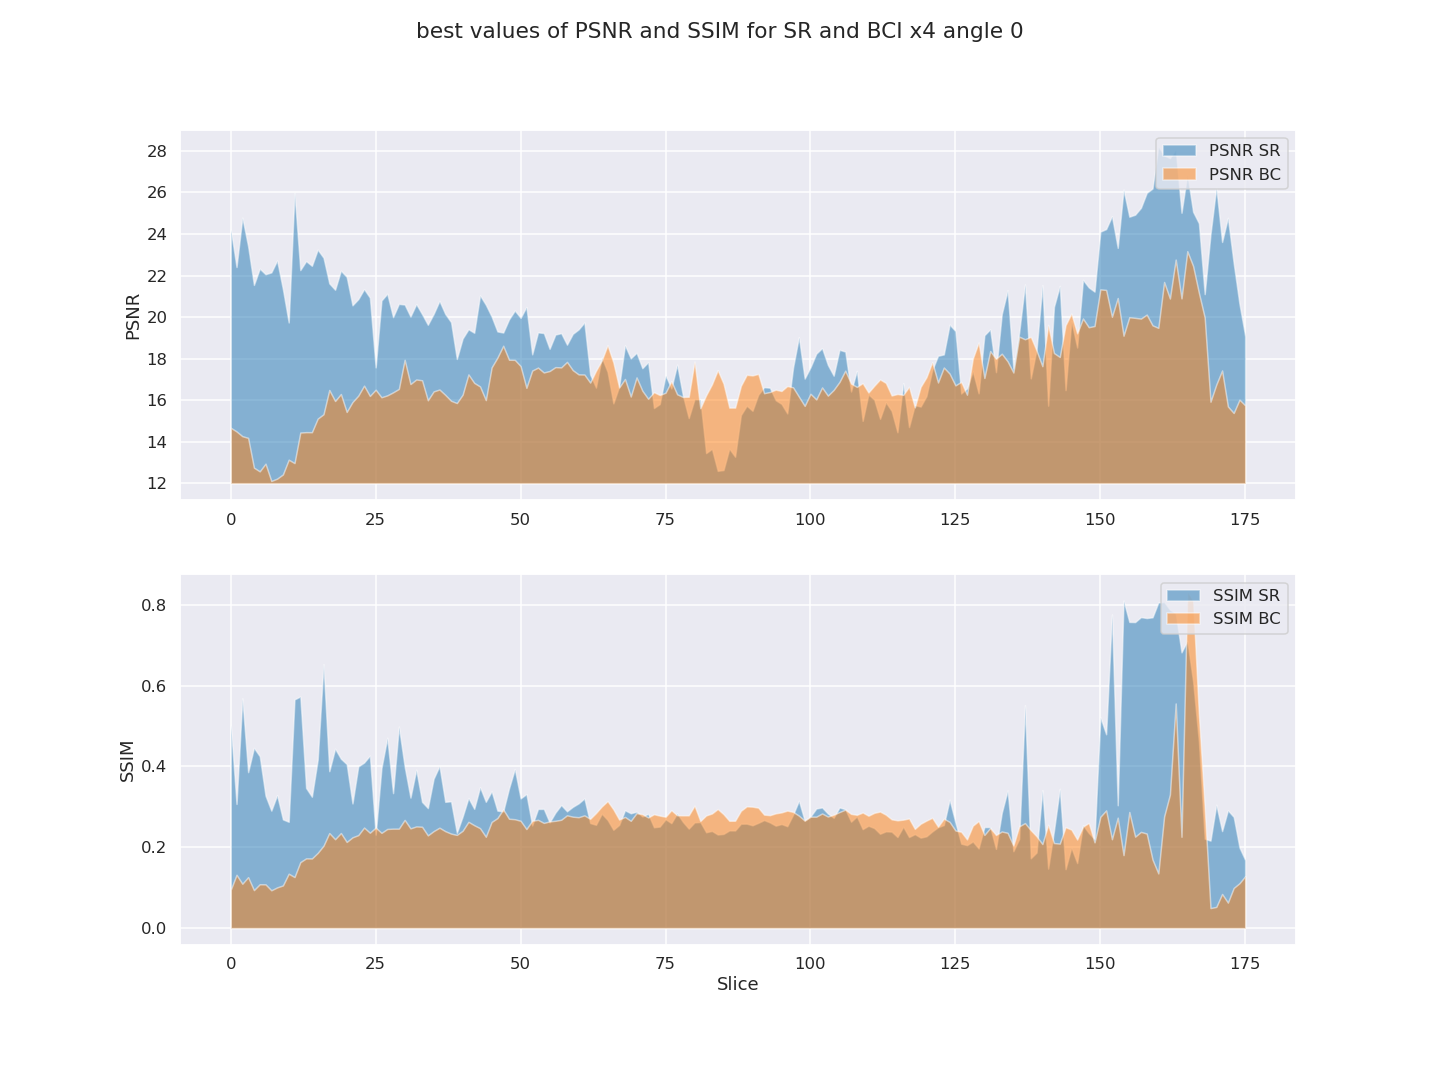
\includegraphics[scale=0.22]{images/PSNR-SSIM_sr-bc_x4_000.png}
 \end{figure}
\end{frame}

\begin{frame}
\frametitle{WDSR results per slice}
   \begin{figure}
  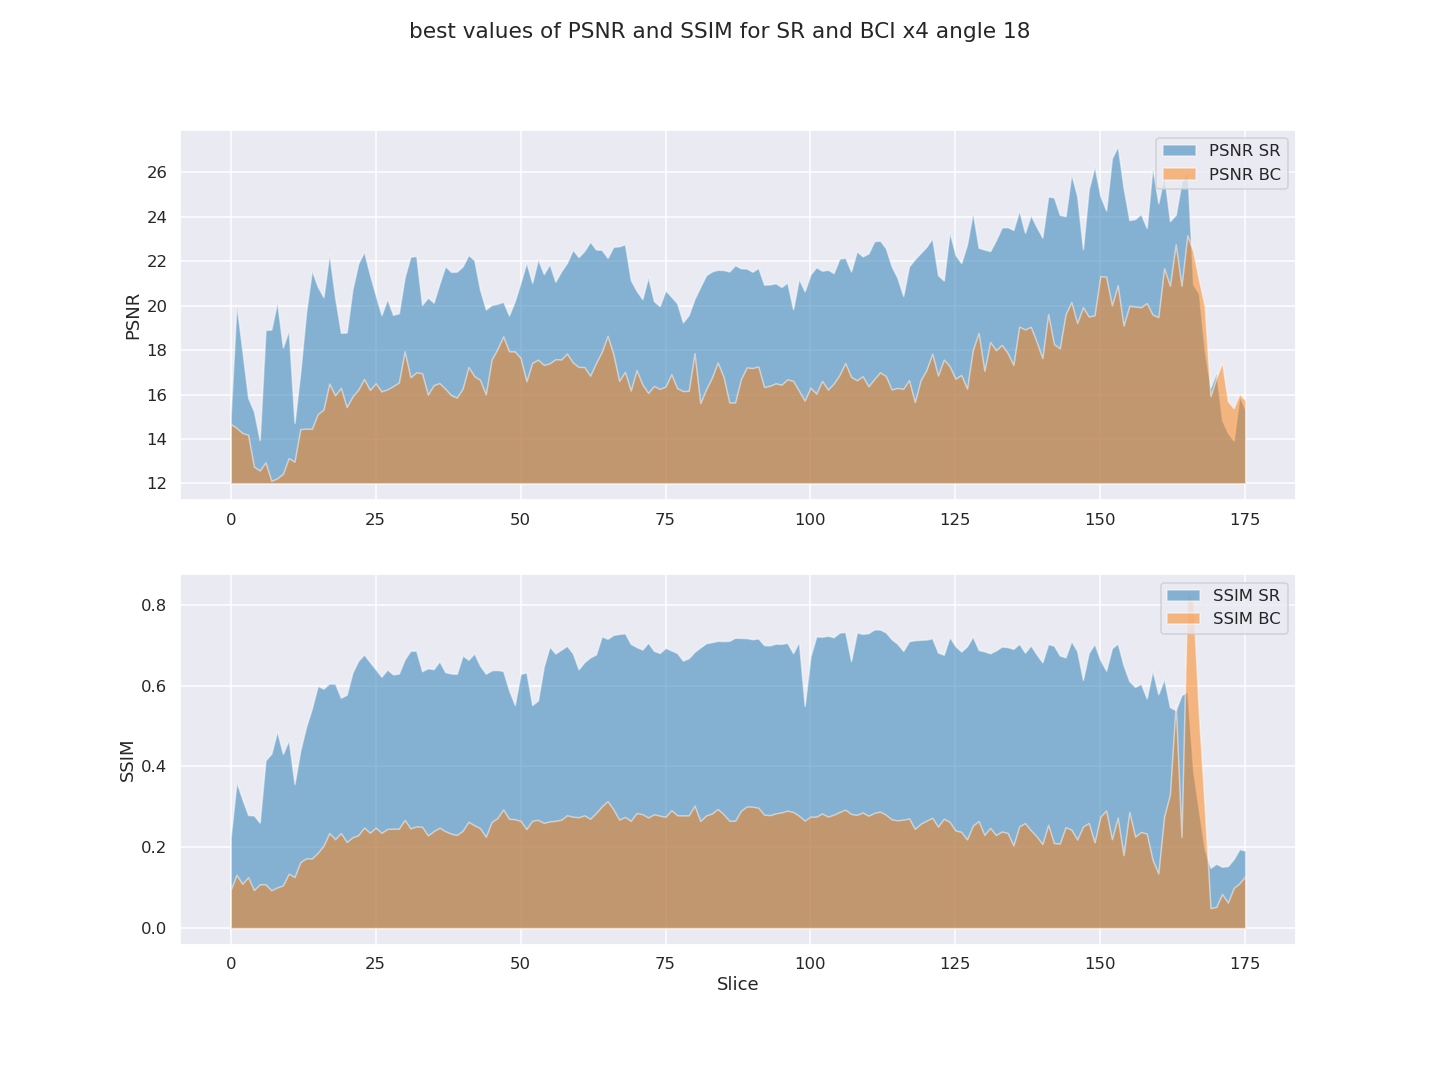
\includegraphics[scale=0.22]{images/PSNR-SSIM_sr-bc_x4_018.png}
 \end{figure}
\end{frame}

\begin{frame}
 \frametitle{WDSR comparisons between angles : 0 and 18}
 \begin{figure}
  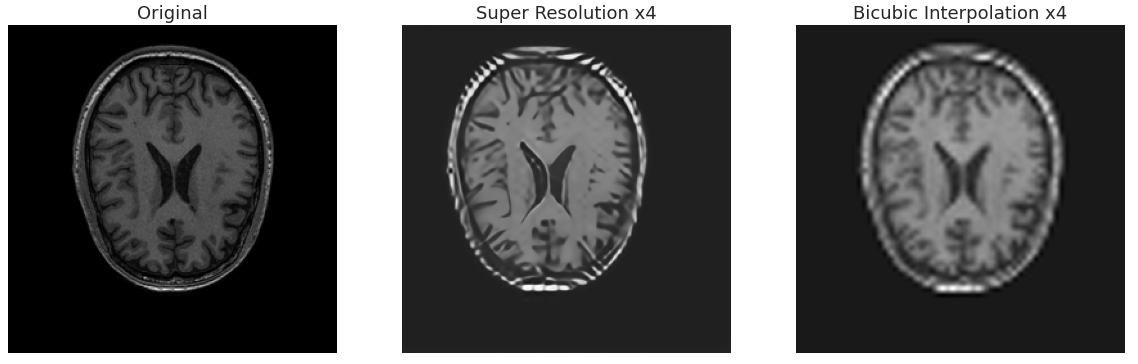
\includegraphics[scale=0.29]{images/ref_case01015_t1_4lr_103_000.png}
  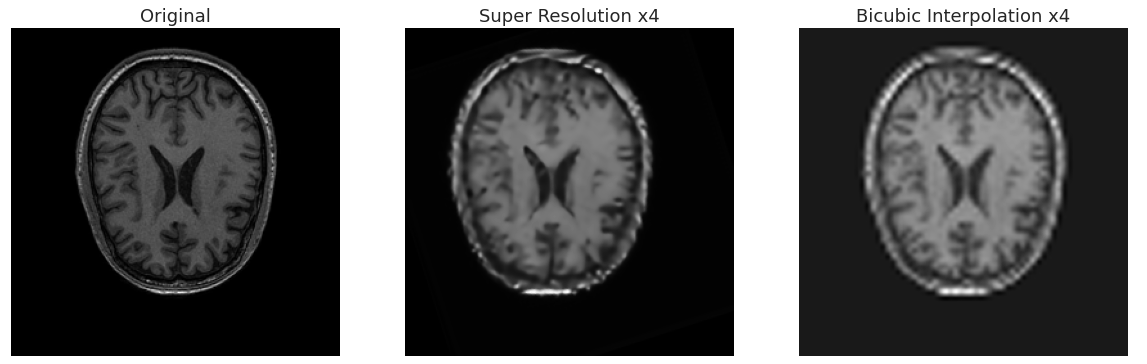
\includegraphics[scale=0.29]{images/ref_case01015_t1_4lr_103_018.png}
 \end{figure}

\end{frame}



\begin{frame}
 \frametitle{EDSR absolute difference per angle}
 \begin{figure}
  \hspace{-2.4cm}
  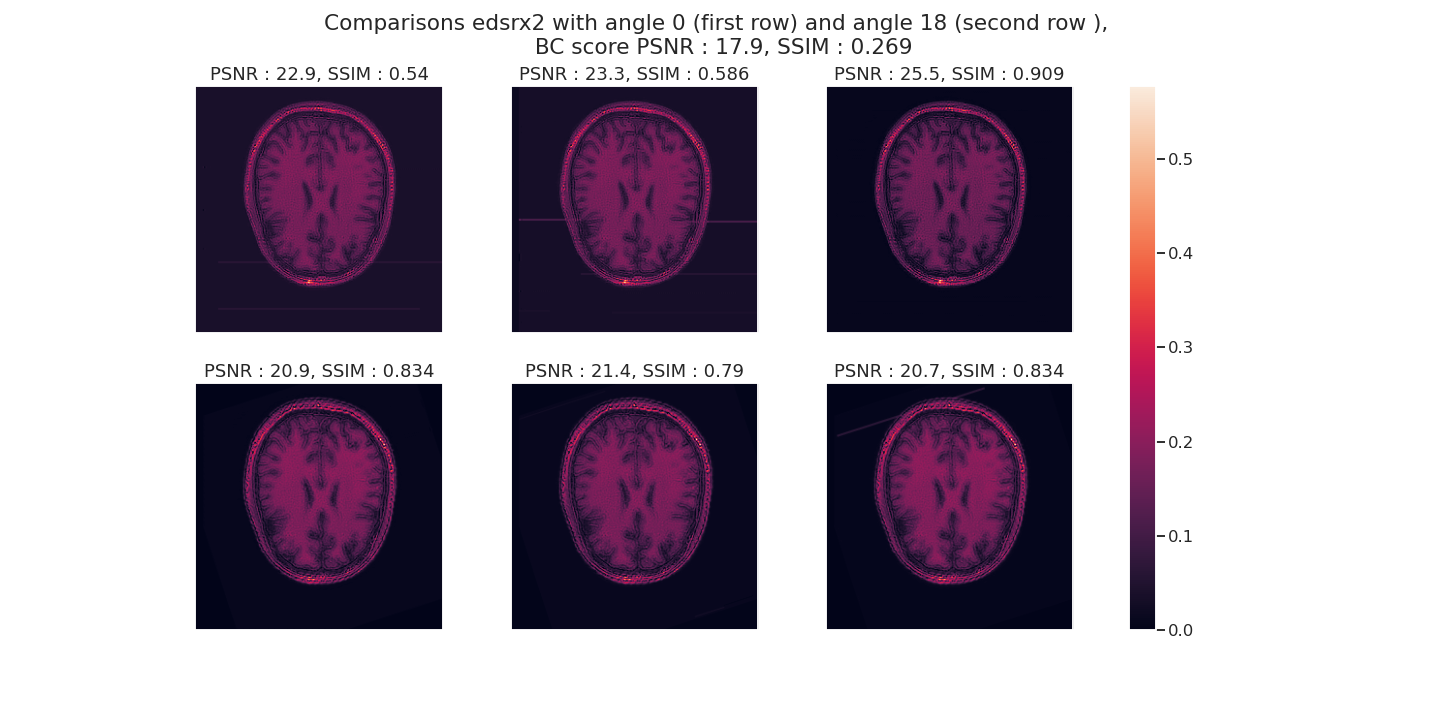
\includegraphics[scale=0.26]{images/edsrx2_diff_108_000_018.png}
 \end{figure}
\end{frame}


\begin{frame}
\frametitle{WDSR absolute difference per angle}
\begin{figure}
 \hspace{-2.4cm}
 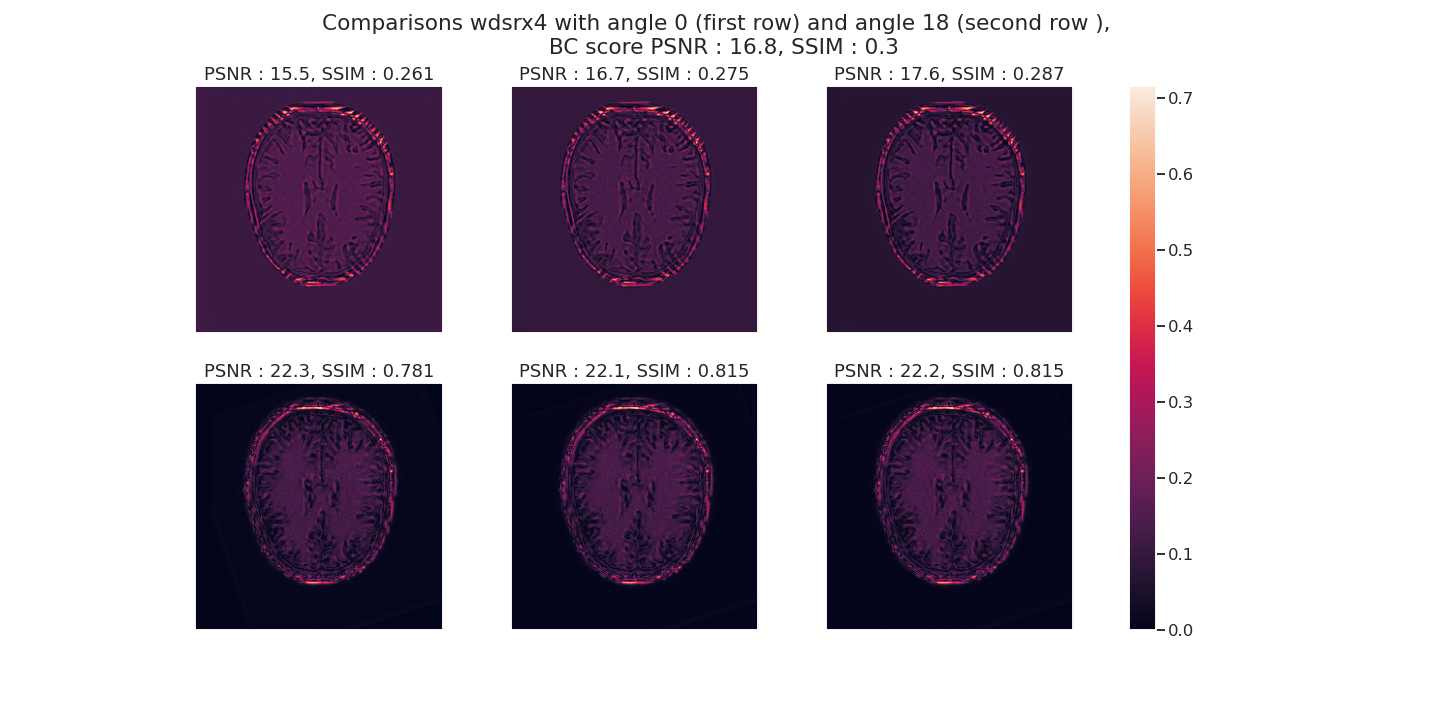
\includegraphics[scale=0.26]{images/wdsrx4_diff_108_000_018.png}
\end{figure}
\end{frame}

\end{document}
